\documentclass{article}
\usepackage[a4paper, total={6in, 8in}]{geometry}
\usepackage{listings}
\usepackage{xcolor}
\usepackage{graphicx}
\usepackage{verbatim}
\usepackage{hyperref}
\usepackage{url}
\usepackage[utf8]{inputenc}
\usepackage{float}

\lstset{
  basicstyle=\ttfamily\footnotesize,
  keywordstyle=\color{blue}\bfseries,
  commentstyle=\color{green!50!black},
  stringstyle=\color{red},
  numbers=left,
  numberstyle=\tiny\color{gray},
  stepnumber=1,
  numbersep=5pt,
  tabsize=2,
  breaklines=true,
  breakatwhitespace=false,
  showspaces=false,
  showstringspaces=false,
  showtabs=false,
  frame=single,
  rulecolor=\color{black},
  captionpos=b,
  language=C++,
  morekeywords={},
}

\begin{document}

\title{\textbf{Modern Tetris Implementation:\\Object-Oriented Design \& Documentation \\ - Final Version }}
\author{By CS23B1023 Athidathan K}
\date{\today}
\maketitle
\tableofcontents
\newpage
\section{Overview}

This documentation provides an overview of the Tetris project, explaining its structure, specifications, and how various Object-Oriented Programming (OOP) concepts are incorporated, including encapsulation, abstraction, inheritance, polymorphism, operator overloading, and plans for future use of templates and virtual functions.

The Tetris project is implemented in C++ using the Raylib graphics library. The game simulates the classic Tetris gameplay, where different shaped blocks fall into a grid, and the player manipulates them to form complete rows.
\subsection{Changes from Mid-Semester Version}
\begin{itemize}
    \item \textbf{Polymorphism}:
    \begin{itemize}
        \item Introduced an abstract class \texttt{GameMode} to facilitate common interface for different game modes.
        \item Created derived classes \texttt{SinglePlayer} and \texttt{TwoPlayer}.
    \end{itemize}
    \item \textbf{Main Function}:
    \begin{itemize}
        \item Added a title screen for game mode selection.
        \item Reworked main logic to support different game modes using polymorphism.
        \item Implemented exception handling.
        \item Added background music.
        \item Introduced game over logic and a game over screen.
    \end{itemize}
    \item \textbf{Game Class}:
    \begin{itemize}
        \item Moved UI drawing logic to the \texttt{Game} class's \texttt{Draw} function.
        \item Added support for offset parameters in the \texttt{Draw} function.
        \item Added Rotate and Clear Sounds.
    \end{itemize}
    \item \textbf{Grid Class}:
    \begin{itemize}
        \item Added support for offset parameters in the \texttt{Draw} function for multiple game grids.
    \end{itemize}
\end{itemize}

These changes significantly enhance the flexibility, maintainability, and functionality of the Tetris project, providing a robust foundation for future development and additional game modes.
\newpage
\section{Project Structure}

\begin{verbatim}
.vscode/
build/
Font/
    Handjet.ttf
lib/
    raylib.h
Screenshots/
Sounds/
    clear.mp3
    music.mp3
    rotate.mp3
src/
    block.cpp
    block.h
    blocks.h
    colors.cpp
    colors.h
    game_mode.h
    game.cpp
    game.h
    grid.cpp
    grid.h
    main.cpp
    position.cpp
    position.h
    single_player.cpp
    single_player.h
    two_player.cpp
    two_player.h
Makefile
Documentation.tex
main.code-workspace
\end{verbatim}

\section{Classes and Files}

\subsection{\texttt{Position} Class (\texttt{src/position.h}, \texttt{src/position.cpp})}

Represents the position of a block in the grid.

\begin{lstlisting}[language=C++]
class Position {
public:
    int row;
    int column;
    Position(int row, int column);
    Position operator+(const Position& other) const;
};
\end{lstlisting}

\subsection{\texttt{Block} Class Hierarchy (\texttt{src/block.h}, \texttt{src/block.cpp}, \texttt{src/blocks.cpp})}
\subsubsection{Base \texttt{Block} Class}
\textbf{Encapsulation}: The \texttt{Block} class encapsulates the properties and behaviors of a Tetris block.

\begin{lstlisting}[language=C++]
class Block {
public:
    Block();
    void Draw(int offsetX, int offsetY);
    void Move(int rows, int columns);
    void Rotate();
    void UndoRotation();
    std::vector<Position> GetCellPositions();
protected:
    int id;
    int rotationState;
    int rowOffset;
    int columnOffset;
    std::map<int, std::vector<Position>> cells;
    int cellSize;
    std::vector<Color> colors;
};
\end{lstlisting}

\textbf{Example}: The \texttt{Block} class manages its state internally and provides public methods for interaction, demonstrating encapsulation.

\subsubsection{Derived Block Classes (\texttt{src/blocks.cpp})}

\textbf{Inheritance}: Multiple classes (\texttt{LBlock}, \texttt{JBlock}, \texttt{IBlock}, \texttt{OBlock}, \texttt{SBlock}, \texttt{TBlock}, \texttt{ZBlock}) inherit from the \texttt{Block} class.

\textbf{Example}:

\begin{lstlisting}[language=C++]
// src/blocks.cpp

#include "block.h"

// LBlock class inheriting from Block
class LBlock : public Block {
public:
    LBlock() {
        id = 1;
        cells[0] = {Position(0, 2), Position(1, 0), Position(1, 1), Position(1, 2)};
        cells[1] = {Position(0, 1), Position(1, 1), Position(2, 1), Position(2, 2)};
        cells[2] = {Position(1, 0), Position(1, 1), Position(1, 2), Position(2, 0)};
        cells[3] = {Position(0, 0), Position(0, 1), Position(1, 1), Position(2, 1)};
        Move(0, 3);
    }
};

// Other block classes (JBlock, IBlock, OBlock, SBlock, TBlock, ZBlock) defined similarly
\end{lstlisting}

Each derived class initializes its specific shape by setting up the \texttt{cells} member variable inherited from the \texttt{Block} class.

\subsection{\texttt{Grid} Class (\texttt{src/grid.h}, \texttt{src/grid.cpp})}

Represents the game grid where the blocks are placed. Manages the grid state, drawing, and clearing full rows.

\begin{lstlisting}[language=C++]
// src/grid.h

#pragma once
#include <vector>
#include <raylib.h>

class Grid {
public:
    Grid();
    void Initialize();
    void Print();
    void Draw();
    bool IsCellOutside(int row, int column);
    bool IsCellEmpty(int row, int column);
    int ClearFullRows();
private:
    int grid[20][10];
    int numRows;
    int numCols;
    int cellSize;
    std::vector<Color> colors;
    bool IsRowFull(int row);
    void ClearRow(int row);
    void MoveRowDown(int row, int numRows);

friend class Game;
};
\end{lstlisting}

\subsection{\texttt{Game} Class (\texttt{src/game.h}, \texttt{src/game.cpp})}

Controls the overall game logic.

\textbf{Abstraction}: Provides simplified methods to handle game mechanics like input handling and block movement.

\begin{lstlisting}[language=C++]
// src/game.h

#pragma once
#include "grid.h"
#include "block.h"
#include "raylib.h"

class Game {
public:
    Game(int playerNumber = 1);
    ~Game();
    void Draw(int offsetX = 0, int offsetY = 0);
    void HandleInput();
    void HandleInputPlayer2();
    void MoveBlockDown();
    void DrawGameOverScreen(Game& winner);
    void Reset();
    bool gameOver;
    int score;
    int playerNumber;
    Font font;
private:
    void MoveBlockLeft();
    void MoveBlockRight();
    Block GetRandomBlock();
    std::vector<Block> GetAllBlocks();
    bool IsBlockOutside();
    void RotateBlock();
    void LockBlock();
    bool BlockFits();
    void UpdateScore(int linesCleared, int moveDownPoints);
    Grid grid;
    std::vector<Block> blocks;
    Block currentBlock;
    Block nextBlock;
    Sound rotateSound;
    Sound clearSound;
};
\end{lstlisting}

\subsection{\texttt{GameMode} Abstract Class (\texttt{src/game\_mode.h})}
Defines a common interface for different game modes.
\textbf{Polymorphism}: Uses virtual functions to allow derived classes to provide specific implementations for different game modes.

\begin{lstlisting}[language=C++]
// src/game_mode.h

#pragma once
#include "game.h"

class GameMode {
public:
    virtual void HandleInput() = 0;
    virtual void Update() = 0;
    virtual void Draw() = 0;
    virtual bool IsGameOver() const = 0;
    virtual ~GameMode() = default;
    virtual Game* GetWinner() = 0;
    virtual int getWinnerScore() = 0;
    virtual void Reset() = 0;
};
\end{lstlisting}

\subsection{\texttt{SinglePlayer} Class (\texttt{src/single\_player.h}, \texttt{src/single\_player.cpp})}

Implements the single-player game mode.

\textbf{Inheritance}: Inherits from \texttt{GameMode} and provides specific implementations for single-player mode.

\begin{lstlisting}[language=C++]
// src/single_player.h

#pragma once
#include "game_mode.h"

class SinglePlayer : public GameMode {
public:
    SinglePlayer();
    void HandleInput() override;
    void Update() override;
    void Draw() override;
    bool IsGameOver() const override;
    ~SinglePlayer() override = default;
    Game* GetWinner() override;
    int getWinnerScore() override { return GetWinner()->score; }
    void Reset() override { game.Reset(); }
private:
    Game game;
};
\end{lstlisting}
\subsection{\texttt{TwoPlayer} Class (\texttt{src/two\_player.h}, \texttt{src/two\_player.cpp})}

Implements the two-player game mode.

\textbf{Inheritance}: Inherits from \texttt{GameMode} and provides specific implementations for two-player mode.

\begin{lstlisting}[language=C++]
// src/two_player.h

#pragma once
#include "game_mode.h"

class TwoPlayer : public GameMode {
public:
    TwoPlayer();
    void HandleInput() override;
    void Update() override;
    void Draw() override;
    bool IsGameOver() const override;
    Game* GetWinner() override;
    int getWinnerScore() override { return GetWinner()->score; }
    void Reset() override { 
        player1Game.Reset(); 
        player2Game.Reset(); 
    }
private:
    Game player1Game;
    Game player2Game;
};
\end{lstlisting}

\begin{lstlisting}[language=C++]
// src/two_player.cpp

#include "two_player.h"

TwoPlayer::TwoPlayer() : player1Game(1), player2Game(2) {
    // Initialize the two-player games
}

void TwoPlayer::HandleInput() {
    player1Game.HandleInput();
    player2Game.HandleInputPlayer2();
}

void TwoPlayer::Update() {
    player1Game.MoveBlockDown();
    player2Game.MoveBlockDown();
}

void TwoPlayer::Draw() {
    player1Game.Draw(0, 0);
    player2Game.Draw(500, 0);
}

bool TwoPlayer::IsGameOver() const {
    return player1Game.gameOver || player2Game.gameOver;
}

Game* TwoPlayer::GetWinner() {
    if (player1Game.score > player2Game.score) 
        return &player1Game;
    else 
        return &player2Game;
}
\end{lstlisting}
\section{OOP Concepts Incorporated}

\subsection{Encapsulation}

Classes manage their own data and expose functionality through public methods. Access specifiers \texttt{public} and \texttt{private} are used to enforce access control, separating the interface from the implementation.

\textbf{Example}:

In the \texttt{Block} class (\texttt{src/block.h}), data members are declared as \texttt{protected} or \texttt{private}, while member functions that form the interface are declared as \texttt{public}.

\begin{lstlisting}[language=C++]
// src/block.h

class Block {
public:
    Block();
    void Draw(int offsetX, int offsetY);
    void Move(int rows, int columns);
    void Rotate();
    void UndoRotation();
    std::vector<Position> GetCellPositions();
protected:
    int id;
    int rotationState;
    int rowOffset;
    int columnOffset;
    std::map<int, std::vector<Position>> cells;
    int cellSize;
    std::vector<Color> colors;
};
\end{lstlisting}

The implementation of these member functions is separated in the corresponding \texttt{.cpp} file (\texttt{src/block.cpp}), keeping the interface clean and promoting encapsulation.

\subsection{Abstraction}

Abstraction is achieved by using header files to define class interfaces. The implementation details are hidden in the \texttt{.cpp} files, allowing users of the classes to interact with them without needing to understand the internal workings.

\textbf{Example}:

The \texttt{Game} class interface is defined in \texttt{src/game.h}, abstracting the game mechanics and providing a clear interface for interaction.

\begin{lstlisting}[language=C++]
// src/game.h

class Game {
public:
    Game();
    ~Game();
    void Draw();
    void HandleInput();
    void MoveBlockDown();
    bool gameOver;
    int score;
private:
    // Private member functions and variables
};
\end{lstlisting}

\subsection{Inheritance}

Inheritance is used to create specialized block types from a base \texttt{Block} class. This allows for code reuse and establishes a hierarchical class structure.

\textbf{Class Hierarchy}:

\begin{itemize}
    \item \texttt{Block} (base class)
    \begin{itemize}
        \item \texttt{IBlock}
        \item \texttt{JBlock}
        \item \texttt{LBlock}
        \item \texttt{OBlock}
        \item \texttt{SBlock}
        \item \texttt{TBlock}
        \item \texttt{ZBlock}
    \end{itemize}
\end{itemize}

\textbf{Example}:

\begin{lstlisting}[language=C++]
// src/blocks.cpp

class TBlock : public Block {
public:
    TBlock() {
        id = 6;
        cells[0] = {Position(0, 1), Position(1, 0), Position(1, 1), Position(1, 2)};
        // other rotation states...
        Move(0, 3);
    }
};
\end{lstlisting}

\subsection{Polymorphism}

Polymorphism allows objects to be treated as instances of their base class rather than their actual derived class. This project demonstrates both compile-time and run-time polymorphism.

\subsubsection{Compile-Time Polymorphism}

\textbf{Function Overloading (used)}:

Function overloading is utilized in the project to allow functions with the same name to have different parameter lists.

\begin{lstlisting}[language=C++]
// src/block.h
class Block {
public:
    void Move(int rows, int columns);
    
    // Overloaded Move function
    void Move(const Position& pos);
};
\end{lstlisting}

\textbf{Operator Overloading (used)}:

Operator overloading is implemented in the \texttt{Position} class to simplify position arithmetic.

\begin{lstlisting}[language=C++]
// src/position.cpp

Position Position::operator+(const Position &other) const{
    return Position(row + other.row, column + other.column);
}
\end{lstlisting}

This allows positions to be added using the \texttt{+} operator.

\textbf{Templates (not currently used)}:

Templates are not explicitly used in this project as the data types are consistent, and there's no immediate need for generic programming. However, templates could be implemented for generic data structures or algorithms if needed in future enhancements.

\subsubsection{Run-Time Polymorphism}

\textbf{Virtual Functions (used)}:

Run-time polymorphism is achieved through the use of virtual functions in the `GameMode` abstract class. This allows derived classes to provide specific implementations for different game modes.

\textbf{Example}:

The \texttt{GameMode} Abstract class defines a common interface for different game modes using pure virtual functions. The \texttt{SinglePlayer} and \texttt{TwoPlayer} classes inherit from \texttt{GameMode} and provide specific implementations for these virtual functions.

\begin{lstlisting}[language=C++]
// src/game_mode.h

#pragma once
#include "game.h"

class GameMode {
public:
    virtual void HandleInput() = 0;
    virtual void Update() = 0;
    virtual void Draw() = 0;
    virtual bool IsGameOver() const = 0;
    virtual ~GameMode() = default;
    virtual Game* GetWinner() = 0;
    virtual int getWinnerScore() = 0;
    virtual void Reset() = 0;
};
\end{lstlisting}

\textbf{Derived Classes}:

\begin{lstlisting}[language=C++]
// src/single_player.h

#pragma once
#include "game_mode.h"

class SinglePlayer : public GameMode {
public:
    SinglePlayer();
    void HandleInput() override;
    void Update() override;
    void Draw() override;
    bool IsGameOver() const override;
    ~SinglePlayer() override = default;
    Game* GetWinner() override;
    int getWinnerScore() override { return GetWinner()->score; }
    void Reset() override { game.Reset(); }
private:
    Game game;
};
\end{lstlisting}

\begin{lstlisting}[language=C++]
// src/two_player.h

#pragma once
#include "game_mode.h"

class TwoPlayer : public GameMode {
public:
    TwoPlayer();
    void HandleInput() override;
    void Update() override;
    void Draw() override;
    bool IsGameOver() const override;
    Game* GetWinner() override;
    int getWinnerScore() override { return GetWinner()->score; }
    void Reset() override { 
        player1Game.Reset(); 
        player2Game.Reset(); 
    }
private:
    Game player1Game;
    Game player2Game;
};
\end{lstlisting}

\textbf{Usage in Main Function}:

In the main function, a \texttt{GameMode} pointer is used to refer to either a \texttt{SinglePlayer} or \texttt{TwoPlayer} object, demonstrating run-time polymorphism. This pointer is then used to execute the rest of the gameplay loop logic.
\begin{lstlisting}[language=C++]
// src/main.cpp

int main() {
    try {
        // .. Game initialization 
        
        GameMode* game = nullptr;
        if (mode == 1) {
            game = new SinglePlayer();
        } else if (mode == 2) {
            SetWindowSize(1000, 620); // Adjust window size for two-player mode
            game = new TwoPlayer();
        } else {
            throw std::runtime_error("Invalid game mode selected.");
        }
        // Game logic done using GameMode pointer
        while (!WindowShouldClose()) {   
            if (game->IsGameOver()) {
                // Determine the winner
                Game* winner = game->GetWinner();
                winner->DrawGameOverScreen(*winner);
                // Restart mechanism
                if (IsKeyPressed(KEY_ENTER)) {
                    game->Reset();
                    SeekMusicStream(music, 0);
            }
            } else {
                UpdateMusicStream(music);
                game->HandleInput(); // Run-Time Polymorphism 
                if (EventTriggered(0.2)) 
                    game->Update();
                
                BeginDrawing();
                ClearBackground(BLACK);
                game->Draw();
                EndDrawing();
            } 
        }
        UnloadMusicStream(music);
        game->Reset();
        CloseAudioDevice();
        CloseWindow();
    } catch (const std::exception& e) {
        std::cerr << "Error: " << e.what() << std::endl;
        return EXIT_FAILURE;
    }
    return EXIT_SUCCESS;  
}
\end{lstlisting}
\subsection{Exception Handling}

Exception handling is an important aspect of robust software development. In this Tetris project, exception handling is incorporated to manage errors gracefully and ensure the program can recover from unexpected situations. Below are some key areas where exception handling is implemented:

\subsubsection{Main Function}

The main function includes a try-catch block to handle any exceptions thrown during initialization or game execution. This ensures that any errors are caught and reported, preventing the program from crashing unexpectedly.

\begin{lstlisting}[language=C++]
// src/main.cpp
int main() {
    try {

        // game logic 
        
        GameMode* game = nullptr;
        if (mode == 1) {
            game = new SinglePlayer();
        } else if (mode == 2) {
            SetWindowSize(1000, 620); // Adjust window size for two-player mode
            game = new TwoPlayer();
        } else {
            throw std::runtime_error("Invalid game mode selected.");}

        // game logic 
        
    } catch (const std::exception& e) {
        std::cerr << "Error: " << e.what() << std::endl;
        return EXIT_FAILURE;
    }
    return EXIT_SUCCESS;
}
\end{lstlisting}

\subsubsection{Raylib's Automatic Exception Handling}

Raylib provides automatic exception handling for resource loading, such as fonts, sounds, and textures. When resources are not loaded properly, Raylib functions return default values or handle the errors internally, reducing the need for extensive manual exception handling in the code.

For example, when loading a font or sound, Raylib will handle any issues internally and provide a default value if the resource fails to load. This simplifies the code and ensures that the program can continue running even if some resources are not available.

\textbf{Example}:

\begin{lstlisting}[language=C++]
// src/game.cpp
Game::Game(int playerNumber) {
    grid = Grid();
    blocks = GetAllBlocks();
    currentBlock = GetRandomBlock();
    nextBlock = GetRandomBlock();
    gameOver = false;
    score = 0;
    this->playerNumber = playerNumber;

    // Raylib handles errors internally and provides default values
    font = LoadFontEx("Font/Handjet.ttf", 64, 0, 0);
    rotateSound = LoadSound("Sounds/rotate.wav");
    clearSound = LoadSound("Sounds/clear.wav");
}
\end{lstlisting}

By leveraging Raylib's built-in error handling, the code remains clean and concise, while still ensuring robustness and stability.

\section{Example Code Snippets}

\subsection{Drawing a Block}
The \texttt{Block::Draw} function is responsible for rendering a Tetris block on the screen. It takes two parameters, \texttt{offsetX} and \texttt{offsetY}, which allow for positioning the block at different locations.

\begin{lstlisting}[language=C++]
// src/block.cpp

void Block::Draw(int offsetX, int offsetY) {
    std::vector<Position> tiles = GetCellPositions();
    for (const Position& item : tiles) {
        DrawRectangle(
            item.column * cellSize + offsetX,
            item.row * cellSize + offsetY,
            cellSize - 1, cellSize - 1,
            colors[id]
        );
    }
}
\end{lstlisting}

\textbf{Explanation}:

\begin{itemize}
    \item The \texttt{GetCellPositions()} function retrieves the positions of the block's cells.
    \item The \texttt{DrawRectangle} function is used to draw each cell of the block at the specified offset.
    \item The \texttt{offsetX} and \texttt{offsetY} parameters allow the block to be drawn at different positions on the screen.
\end{itemize}

Demonstrates encapsulation by handling drawing internally.

\subsection{Handling Block Rotation}

The \texttt{Block::Rotate} function updates the rotation state of a Tetris block. This function ensures that the block cycles through its available rotation states.

\begin{lstlisting}[language=C++]
// src/block.cpp

void Block::Rotate() {
    rotationState = (rotationState + 1) % cells.size();
}
\end{lstlisting}

\textbf{Explanation}:

\begin{itemize}
    \item The \texttt{rotationState} variable keeps track of the current rotation state of the block.
    \item The rotation state is updated by incrementing it and taking the modulus with the number of rotation states.
    \item This ensures that the rotation state cycles through the available states.
\end{itemize}

Shows how the block manages its rotation state.

\subsection{Moving Blocks Down Automatically}

The following code snippet demonstrates how the game logic moves the current block down at regular intervals, simulating gravity.

\begin{lstlisting}[language=C++]
// src/main.cpp

if (EventTriggered(0.2)) { // Game speed is 0.2 seconds
    game->MoveBlockDown();
}
\end{lstlisting}

\textbf{Explanation}:

\begin{itemize}
    \item The \texttt{EventTriggered} function checks if the specified interval (0.2 seconds) has passed.
    \item If the interval has passed, the \texttt{MoveBlockDown} function is called to move the current block down.
    \item This ensures that the block moves down at regular intervals, simulating gravity.
\end{itemize}

Demonstrates how the game logic moves the current block down at regular intervals.

\subsection{Handling Input for Two Players}

The \texttt{TwoPlayer::HandleInput} function is responsible for handling input separately for two players in a two-player game mode. Player 1 uses the WASD keys for control, while Player 2 uses the arrow keys.

\begin{lstlisting}[language=C++]
// src/two_player.cpp

void TwoPlayer::HandleInput() {
    player1Game.HandleInput();
    player2Game.HandleInputPlayer2();
}
\end{lstlisting}

\begin{lstlisting}[language=C++]
// src/game.cpp

void Game::HandleInput() {
    // Player 1 controls
    if (IsKeyPressed(KEY_A)) MoveBlockLeft();
    if (IsKeyPressed(KEY_D)) MoveBlockRight();
    if (IsKeyPressed(KEY_W)) RotateBlock();
    if (IsKeyPressed(KEY_S))  {
        MoveBlockDown();
        MoveBlockDown();
        UpdateScore(0, 2);}
}

void Game::HandleInputPlayer2() {
    // Player 2 controls
    if (IsKeyPressed(KEY_LEFT)) MoveBlockLeft();
    if (IsKeyPressed(KEY_RIGHT)) MoveBlockRight();
    if (IsKeyPressed(KEY_UP)) RotateBlock();
    if (IsKeyPressed(KEY_DOWN)) {
        MoveBlockDown();
        MoveBlockDown();
        UpdateScore(0, 2);}
}

\end{lstlisting}

\textbf{Explanation}:

\begin{itemize}
    \item The \texttt{HandleInput} function for \texttt{player1Game} handles input for Player 1 using the WASD keys.
    \item The \texttt{HandleInputPlayer2} function for \texttt{player2Game} handles input for Player 2 using the arrow keys.
    \item This ensures that input is handled separately for each player in a two-player game.
\end{itemize}

Demonstrates how input is handled separately for two players, with Player 1 using the WASD keys and Player 2 using the arrow keys.
\subsection{Drawing the Game Using \texttt{Game::Draw(int offsetX, int offsetY)}}

The \texttt{Game::Draw} function is responsible for rendering the game state on the screen. It takes two parameters, \texttt{offsetX} and \texttt{offsetY}, which allow for positioning the game grid and UI elements at different locations. This is particularly useful for multiplayer modes where multiple game grids need to be displayed side by side.

\begin{lstlisting}[language=C++]
// src/game.cpp

void Game::Draw(int offsetX, int offsetY) {
    grid.Draw(offsetX, offsetY);

    // Draw the current block
    currentBlock.Draw(offsetX + 11, offsetY + 11);

    // Draw the UI elements
    DrawTextEx(font, "Score", {(float)(365 + offsetX), (float)(15 + offsetY)}, 38, 2, WHITE);
    char playerText[10];
    sprintf(playerText, "Player %d", playerNumber);
    DrawTextEx(font, playerText, {(float)(365 + offsetX), (float)(500 + offsetY)}, 38, 2, WHITE);
    DrawTextEx(font, "Next", {(float)(370 + offsetX), (float)(175 + offsetY)}, 38, 2, WHITE);
    DrawRectangleRounded({(float)320 + offsetX, (float)55 + offsetY, 170, 60}, 0.3, 6, darkGrey);
    char scoreText[10];
    sprintf(scoreText, "%d", score);
    Vector2 textSize = MeasureTextEx(font, scoreText, 38, 2);
    DrawTextEx(font, scoreText, {(float)offsetX + 320 + (170 - textSize.x) / 2, (float)offsetY + 65}, 38, 2, WHITE);
    DrawRectangleRounded({(float)320 + offsetX, (float)215 + offsetY, 170, 180}, 0.3, 6, darkGrey);

    // Preview the next block
    int previewX, previewY;
    switch (nextBlock.id) {
        case 3:
            previewX = offsetX + 255;
            previewY = offsetY + 290;
            break;
        case 4:
            previewX = offsetX + 255;
            previewY = offsetY + 280;
            break;
        default:
            previewX = offsetX + 270;
            previewY = offsetY + 270;
            break;
    }
    nextBlock.Draw(previewX, previewY);
}
\end{lstlisting}

\textbf{Explanation}:

\begin{itemize}
    \item The \texttt{grid.Draw(offsetX, offsetY)} call renders the game grid at the specified offset.
    \item The \texttt{currentBlock.Draw(offsetX + 11, offsetY + 11)} call draws the current block with a slight offset to align it within the grid.
    \item UI elements, such as the score, player number, and next block preview, are drawn using the \texttt{DrawTextEx} and \texttt{DrawRectangleRounded} functions, positioned based on the provided offsets.
    \item The next block preview is drawn at a specific position based on the block's ID, ensuring it is displayed correctly.
\end{itemize}

This function encapsulates the drawing logic for the game, making it easy to render the game state at different positions on the screen, which is essential for supporting multiplayer modes.

\subsection{Drawing the Game Over Screen}

The \texttt{Game::DrawGameOverScreen} function is responsible for rendering the game over screen, displaying the winner and their score.

\begin{lstlisting}[language=C++]
// src/game.cpp

void Game::DrawGameOverScreen(Game &winner) {
    BeginDrawing();
    ClearBackground(BLACK);
    DrawText("Game Over!", 100, 150, 40, RED);
    DrawText(TextFormat("Winner: Player %d", winner.playerNumber), 100, 220, 30, WHITE);
    DrawText(TextFormat("Score: %d", winner.score), 100, 260, 30, WHITE);
    DrawText("Press ENTER to restart", 100, 320, 20, LIGHTGRAY);
    EndDrawing();
}
\end{lstlisting}

\textbf{Explanation}:

\begin{itemize}
    \item The \texttt{BeginDrawing} and \texttt{EndDrawing} functions are used to start and end the drawing process.
    \item The background is cleared with a black color using \texttt{ClearBackground(BLACK)}.
    \item The game over message, winner information, and restart instructions are drawn using the \texttt{DrawText} and \texttt{TextFormat} functions.
\end{itemize}

Shows how the game over screen is drawn, displaying the winner and their score.

\subsection{Clearing Full Rows in the Grid}

The \texttt{Grid::ClearFullRows} function checks for and clears full rows in the game grid, moving the rows above down as needed.

\begin{lstlisting}[language=C++]
// src/grid.cpp

int Grid::ClearFullRows() {
    int completed = 0;
    for (int row = numRows - 1; row >= 0; row--) {
        if (IsRowFull(row)) {
            ClearRow(row);
            completed++;
        } else if (completed > 0) {
            MoveRowDown(row, completed);
        }
    }
    return completed;
}
\end{lstlisting}

\textbf{Explanation}:

\begin{itemize}
    \item The \texttt{IsRowFull} function checks if a row is completely filled with blocks.
    \item The \texttt{ClearRow} function clears a full row.
    \item The \texttt{MoveRowDown} function moves rows down to fill the cleared space.
    \item The function returns the number of rows cleared.
\end{itemize}

Shows how the grid checks for and clears full rows, moving the rows above down as needed.

\subsection{Updating the Score}

The \texttt{Game::UpdateScore} function updates the player's score based on the number of lines cleared and additional points for moving blocks down.

\begin{lstlisting}[language=C++]
// src/game.cpp

void Game::UpdateScore(int linesCleared, int moveDownPoints){
    if (linesCleared == 1) score += 100;
    else if (linesCleared == 2) score += 200;
    else if (linesCleared == 3) score += 400;
    else if (linesCleared == 4) score += 800;
    // No need for else case as we can't break more than 4 lines at once
    score += moveDownPoints;
}
\end{lstlisting}

\textbf{Explanation}:

\begin{itemize}
    \item The score is updated based on the number of lines cleared.
    \item Additional points are added for moving blocks down.
    \item The function ensures that the score is updated correctly based on the game events.
\end{itemize}

Shows how the score is updated based on the number of lines cleared and additional points for moving blocks down.
\section{Screenshots}

Below are some screenshots demonstrating various aspects of the Tetris project.

\subsection{Title Screen}

\begin{figure}[H]
    \centering
    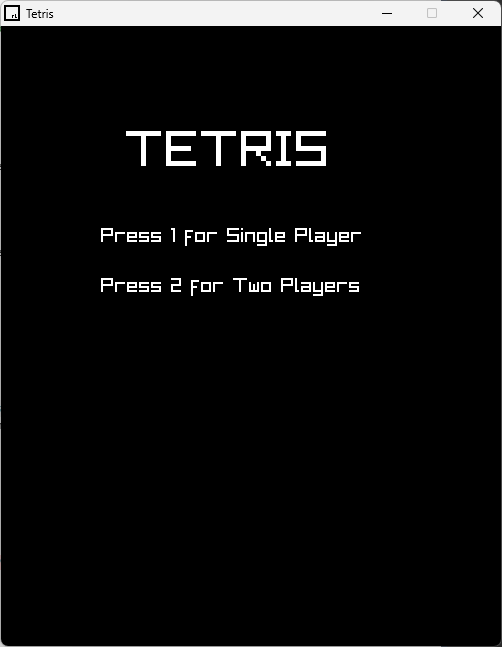
\includegraphics[width=0.8\textwidth]{title_screen.png}
    \caption{Title screen where the player can choose between single-player and two-player modes.}
    \label{fig:title_screen}
\end{figure}

\subsection{Single-Player Mode}

\begin{figure}[H]
    \centering
    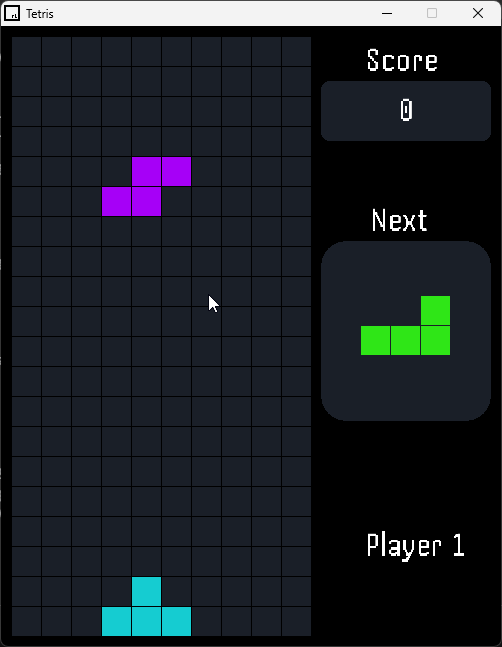
\includegraphics[width=0.8\textwidth]{single_player_mode.png}
    \caption{Single-player mode showing the game grid, falling block, and UI elements.}
    \label{fig:single_player_mode}
\end{figure}

\subsection{Two-Player Mode}

\begin{figure}[H]
    \centering
    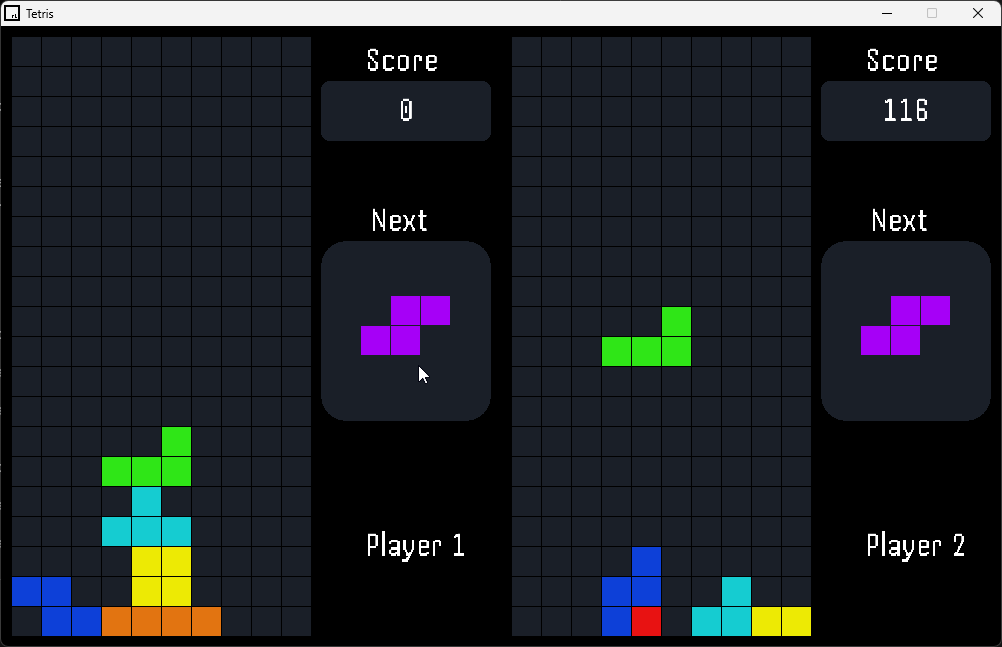
\includegraphics[width=0.8\textwidth]{two_player_mode.png}
    \caption{Two-player mode showing both game grids side by side with UI elements for both players.}
    \label{fig:two_player_mode}
\end{figure}

\subsection{Game Over Screen}

\begin{figure}[H]
    \centering
    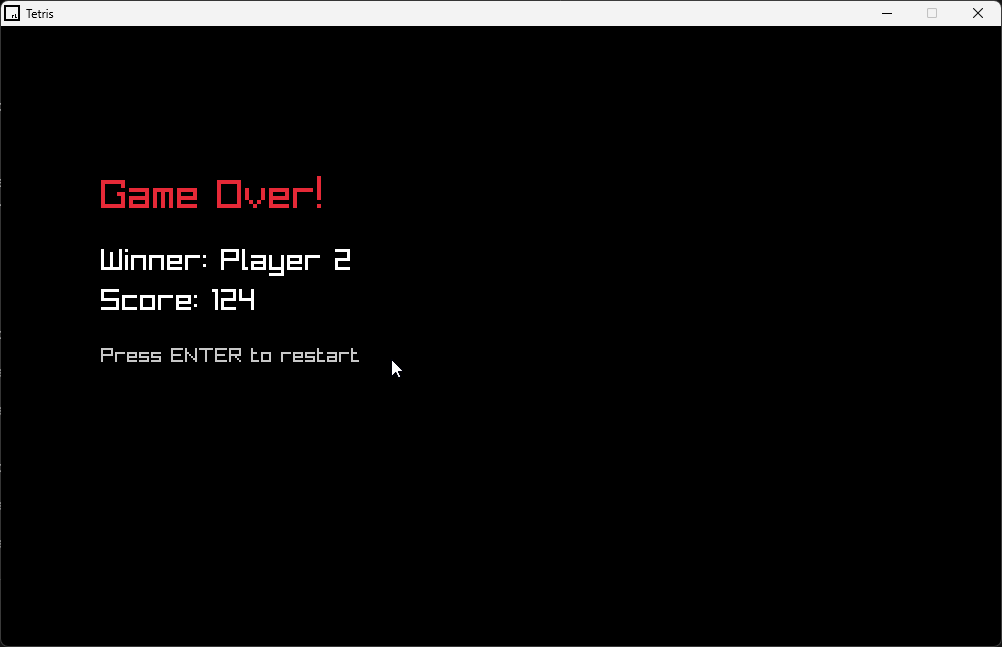
\includegraphics[width=0.8\textwidth]{game_over_screen.png}
    \caption{Game over screen displaying the winner's information and score.}
    \label{fig:game_over_screen}
\end{figure}
\section{Building the Project}

The project is developed in C++ using the Raylib graphics library, and the instructions are tailored for Windows users. This project was developed on Windows 10 using MinGW-w64 as the compiler. The instructions assume a similar setup, but the project can be adapted for other platforms with minor modifications. The project can also be downloaded from my GitHub \url{https://github.com/Athidathan/OOPtetris/}.

\subsection{Requirements}

\begin{itemize}
    \item \textbf{Operating System}: Windows 10 or higher
    \item \textbf{Compiler}: MinGW-w64 (GCC for Windows) or Microsoft Visual Studio
    \item \textbf{Library}: \href{https://www.raylib.com/}{Raylib} (version 4.0 or higher)
    \item \textbf{Make Build System}: MinGW-w64 includes \texttt{mingw32-make} for building the project using the provided \texttt{Makefile}.
\end{itemize}

\subsection{Instructions}

\begin{enumerate}
    \item Install the required compiler and Raylib library.
    \item Open the Command Prompt and navigate to the project directory:
    \begin{lstlisting}
    cd path\to\your\project
    \end{lstlisting}
    \item Compile the project using the provided \texttt{Makefile}:
    \begin{lstlisting}
    mingw32-make
    \end{lstlisting}
    \item Run the game executable:
    \begin{lstlisting}
    game.exe
    \end{lstlisting}
    \item Alternatively, you can use Visual Studio Code to compile and run the project:
    \begin{itemize}
        \item Open the project folder in Visual Studio Code.
        \item Press \texttt{F5} to compile and run the project.
    \end{itemize}
\end{enumerate}

\section{Conclusion}

Working on this Tetris project has been a valuable experience that helped me deepen my understanding of Object-Oriented Programming (OOP) in C++. Through implementing key concepts like encapsulation, abstraction, inheritance, polymorphism, and operator overloading, I’ve developed a better grasp of how OOP principles apply in real-world software development.

This project taught me how to structure a C++ application with classes and inheritance, handle game logic and state management, and use the Raylib graphics library for rendering and input. Using polymorphism with the \texttt{GameMode} abstract class and its derived classes (\texttt{SinglePlayer} and \texttt{TwoPlayer}) highlighted how flexible and scalable this design is, especially when it comes to adding new features like additional game modes.

Implementing exception handling showed me the importance of managing errors properly to make the program more stable and reliable. Raylib’s built-in error handling also made resource management simpler and kept the code cleaner.\\

Looking ahead, there’s plenty of room for improvement and extensibility in this project. I’m particularly interested in exploring features that could help me learn new concepts, like networking, AI, or creating a more polished user interface. These additions would not only make the game more engaging but also give me the opportunity to take on more advanced programming challenges.

Overall, this project has been a solid introduction to OOP in C++ and has given me a better understanding of how to apply these concepts in game development. It’s been a rewarding experience and a great starting point for more complex programming projects.

\newpage
\begin{thebibliography}{9}

\bibitem{raylib}
Raylib Official Website. \url{https://www.raylib.com/}

\bibitem{raylib_tutorials}
Raylib Learning Resources. \url{https://github.com/raysan5/raylib/wiki}

\bibitem{tetris}
Tetris Game. \url{https://en.wikipedia.org/wiki/Tetris}
\end{thebibliography}
\end{document}